\documentclass[9pts]{paper}
\usepackage{graphicx}
\usepackage[margin=0.8in]{geometry}
\usepackage{subfigure}

\begin{document}
%%%%%%%%%%%%%%%%%%%%%%%%%%%%%%%%%%%%%%%%%%%%%
\begin{figure}[ht]
\subfigure[Energy Distribution]{%
\includegraphics[scale=0.4]{8energy_band.pdf}
\label{fig:subfigure81}}
\quad
\subfigure[Compressive Sensing]{%
\includegraphics[scale=0.4]{comp_sen_8}
\label{fig:subfigure82}}
\subfigure[Scalp]{%
\includegraphics[scale=0.4]{ica_8}
\label{fig:subfigure83}}


%
\caption{IC 8}
\label{fig:figure8}
\end{figure}
\begin{figure}
\centering
\includegraphics[width=1\textwidth]{8cwt}
\end{figure}
%%%%%%%%%%%%%%%%%%%%%%%%%%%%%%%%%%%%%%%%%%
\begin{figure}[ht]

\subfigure[Energy Distribution]{%
\includegraphics[scale=0.4]{9energy_band.pdf}
\label{fig:subfigure91}}
\quad
\subfigure[Compressive Sensing]{%
\includegraphics[scale=0.4]{comp_sen_9}
\label{fig:subfigure92}}
\subfigure[Scalp]{%
\includegraphics[scale=0.4]{ica_9}
\label{fig:subfigure93}}

%
\caption{IC 9}
\label{fig:figure}
\end{figure}
\begin{figure}
\centering
\includegraphics[width=1\textwidth]{9cwt}
\end{figure}


\begin{figure}[ht]

\subfigure[Energy Distribution]{%
\includegraphics[scale=0.4]{10energy_band.pdf}
\label{fig:subfigure11}}
\quad
\subfigure[Compressive Sensing]{%
\includegraphics[scale=0.4]{comp_sen_10}
\label{fig:subfigure12}}
\subfigure[Scalp]{%
\includegraphics[scale=0.4]{ica_10}
\label{fig:subfigure13}}

%
\caption{IC 10}
\label{fig:figure11}
\end{figure}
\begin{figure}
\centering
\includegraphics[width=1\textwidth]{10cwt}
\end{figure}

\begin{figure}[ht]

\subfigure[Energy Distribution]{%
\includegraphics[scale=0.4]{11energy_band.pdf}
\label{fig:subfigure121}}
\quad
\subfigure[Compressive Sensing]{%
\includegraphics[scale=0.4]{comp_sen_11}
\label{fig:subfigure122}}
\subfigure[Scalp]{%
\includegraphics[scale=0.4]{ica_11}
\label{fig:subfigure123}}

%
\caption{IC 11}
\label{fig:figure12}
\end{figure}
\begin{figure}
\centering
\includegraphics[width=1\textwidth]{11cwt}
\end{figure}

\begin{figure}[ht]

\subfigure[Energy Distribution]{%
\includegraphics[scale=0.4]{12energy_band.pdf}
\label{fig:subfigure131}}
\quad
\subfigure[Compressive Sensing]{%
\includegraphics[scale=0.4]{comp_sen_12}
\label{fig:subfigure132}}
\subfigure[Scalp]{%
\includegraphics[scale=0.4]{ica_12}
\label{fig:subfigure133}}

%
\caption{IC 12}
\label{fig:figure13}
\end{figure}
\begin{figure}
\centering
\includegraphics[width=1\textwidth]{12cwt}
\end{figure}

\begin{figure}[ht]

\subfigure[Energy Distribution]{%
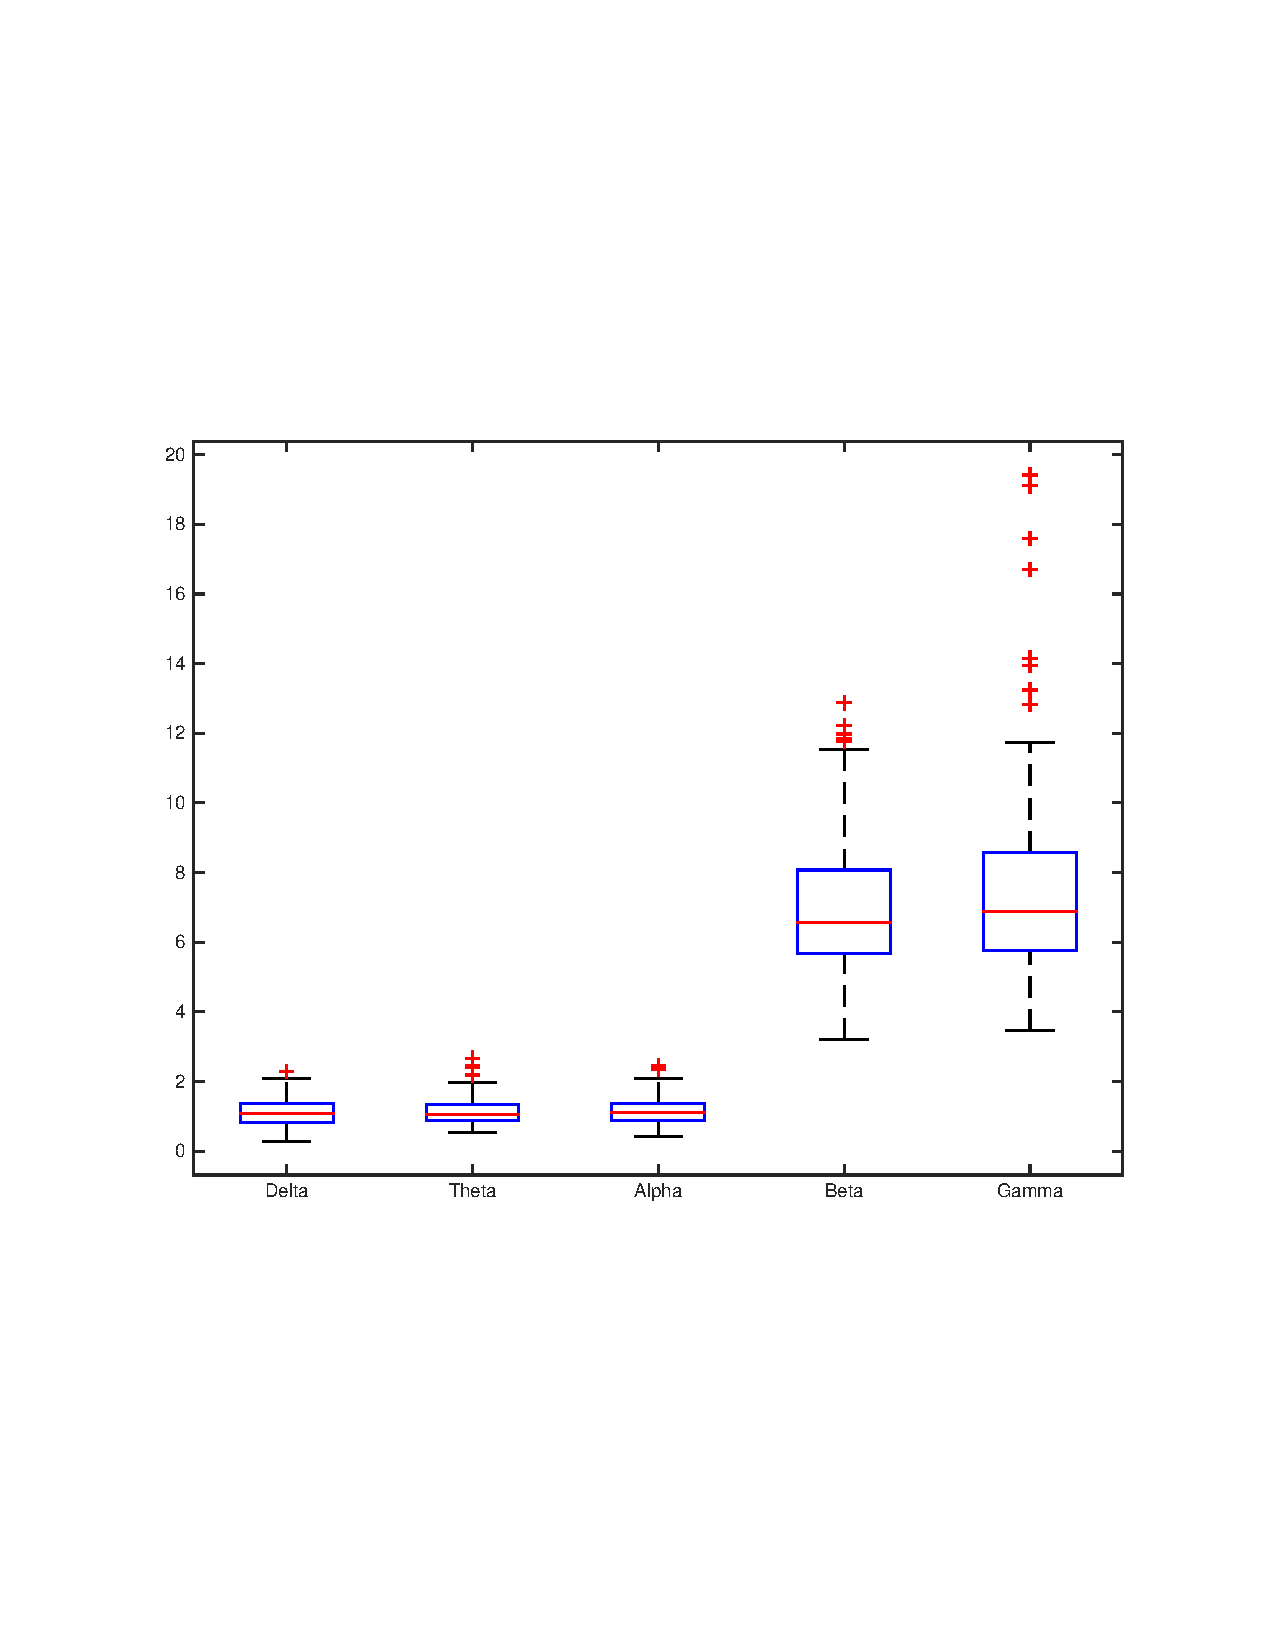
\includegraphics[scale=0.4]{13energy_band.pdf}
\label{fig:subfigure141}}
\quad
\subfigure[Compressive Sensing]{%
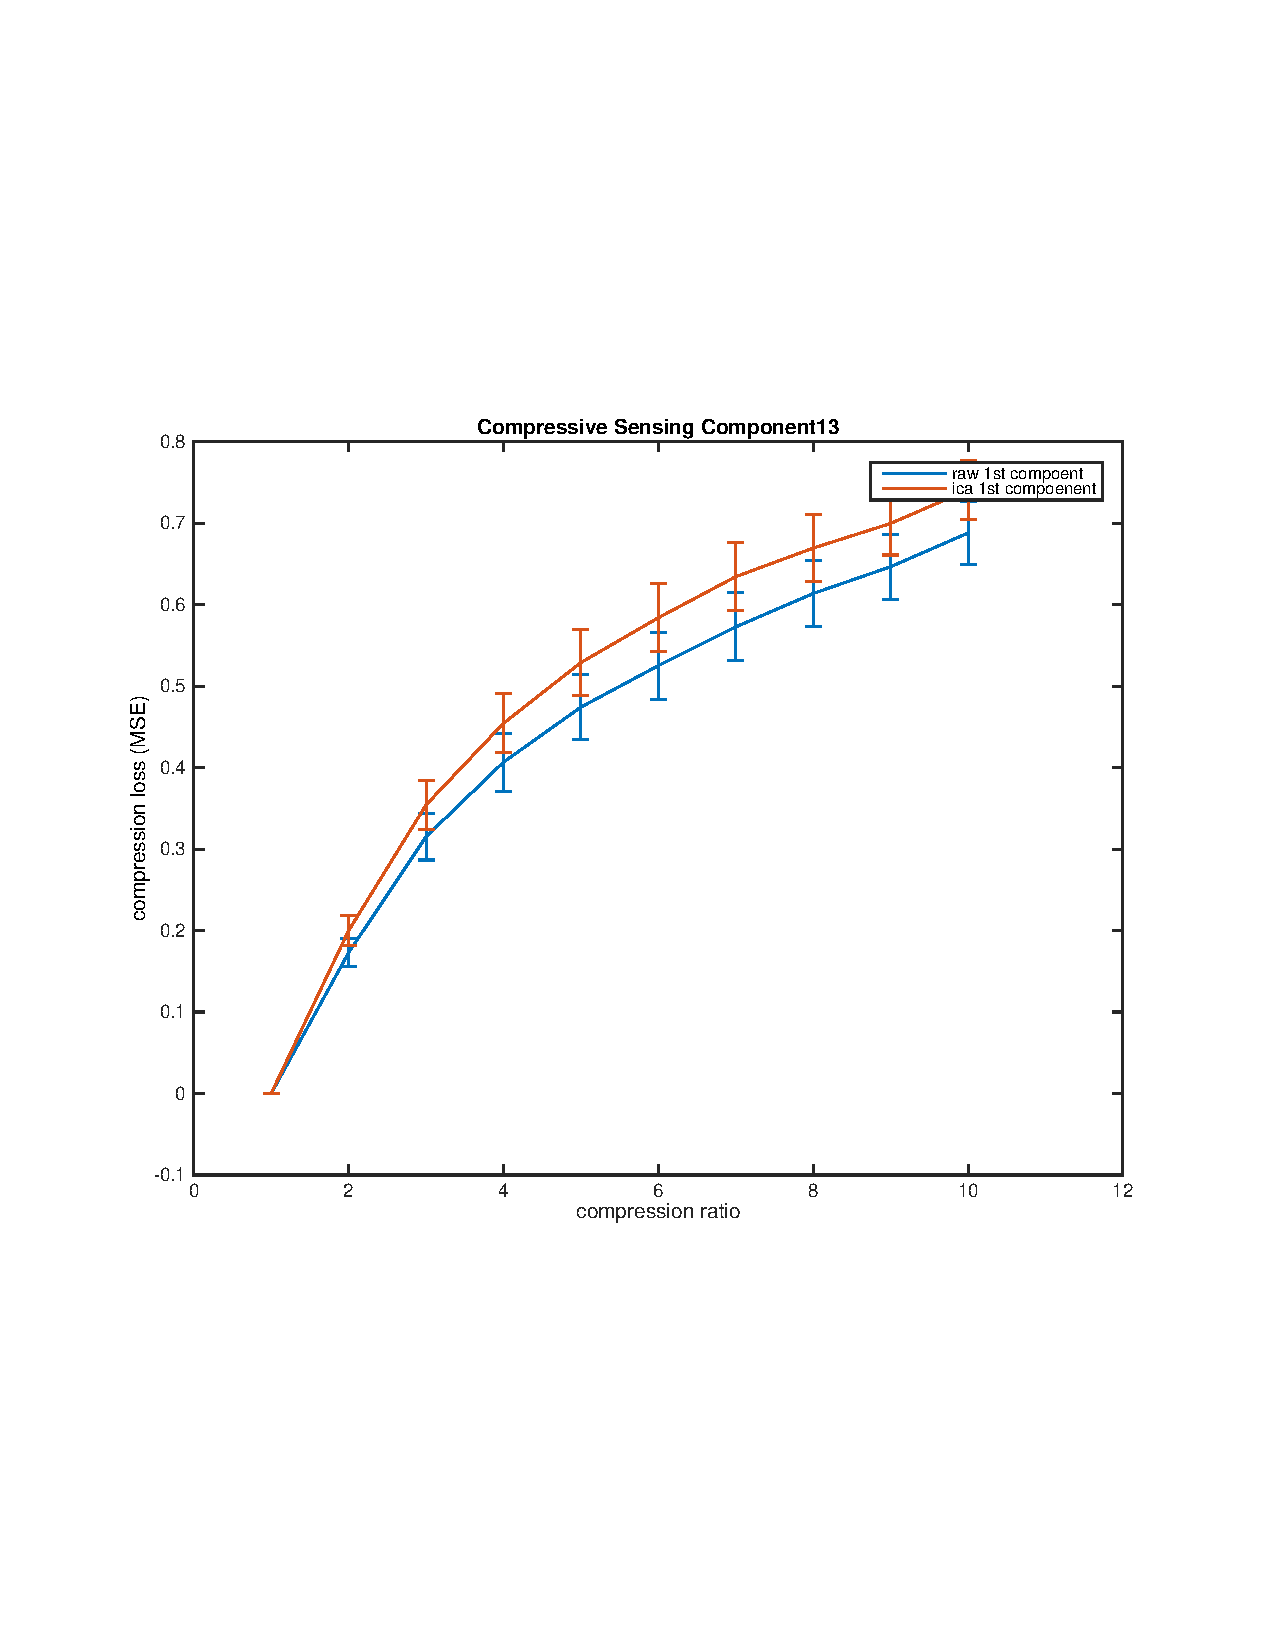
\includegraphics[scale=0.4]{comp_sen_13}
\label{fig:subfigure142}}
\subfigure[Scalp]{%
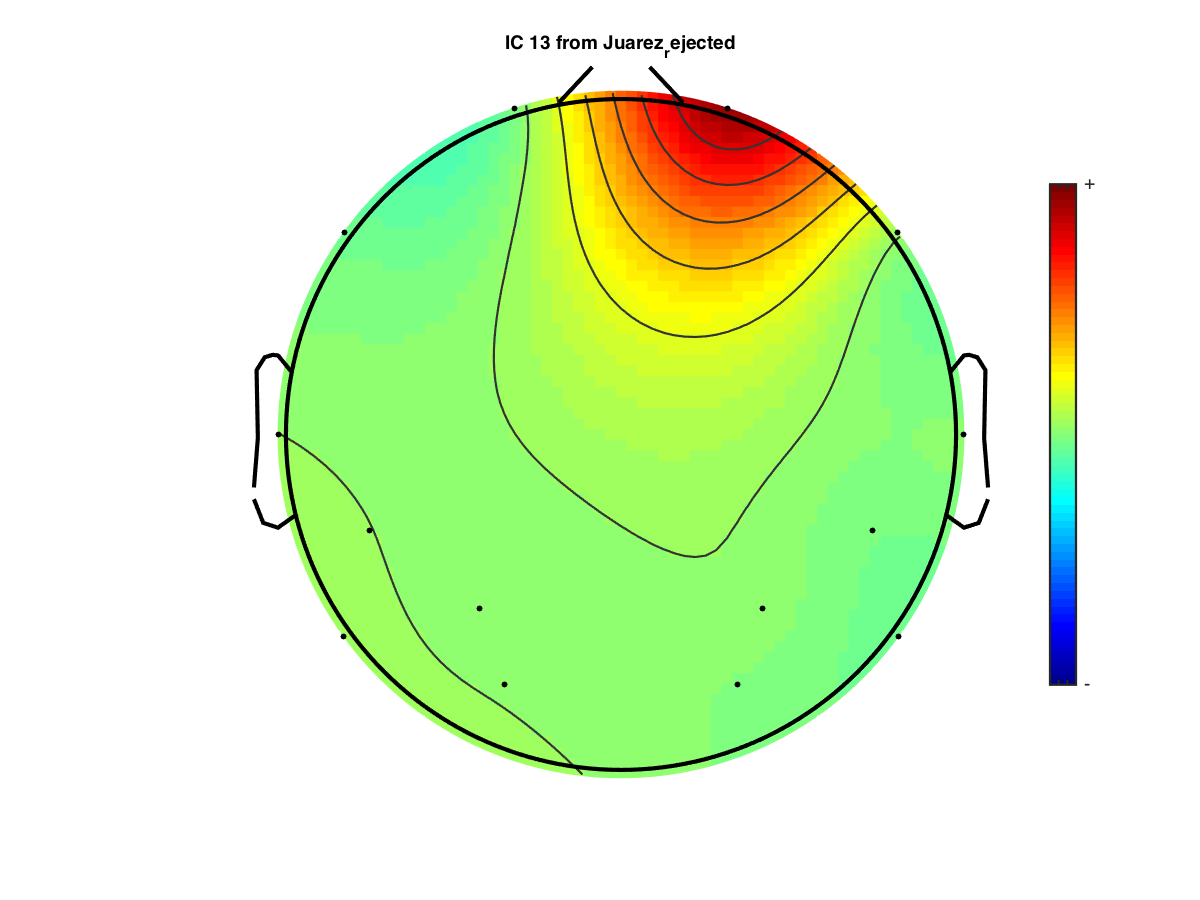
\includegraphics[scale=0.4]{ica_13}
\label{fig:subfigure143}}

%
\caption{IC 13}
\label{fig:figure14}
\end{figure}
\begin{figure}
\centering
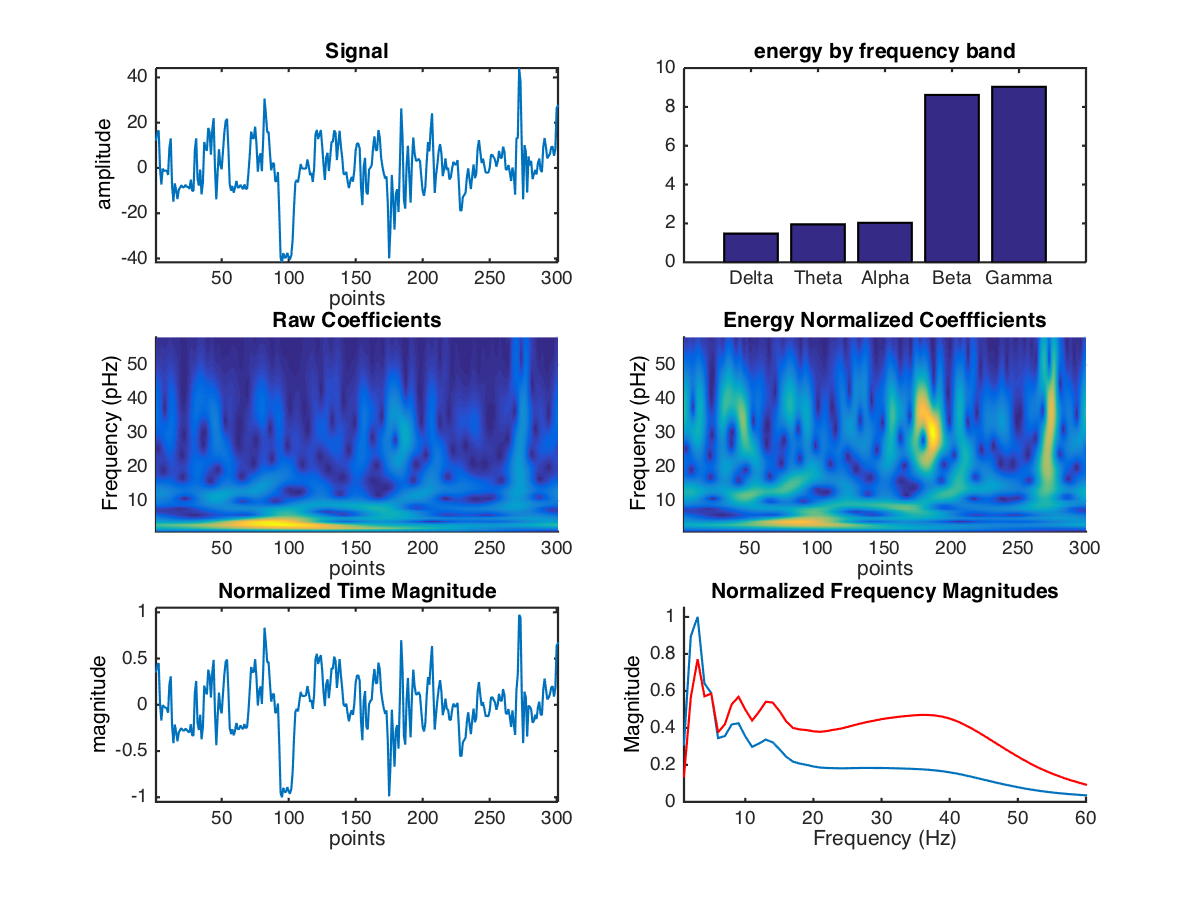
\includegraphics[width=1\textwidth]{13cwt}
\end{figure}

\begin{figure}[ht]

\subfigure[Energy Distribution]{%
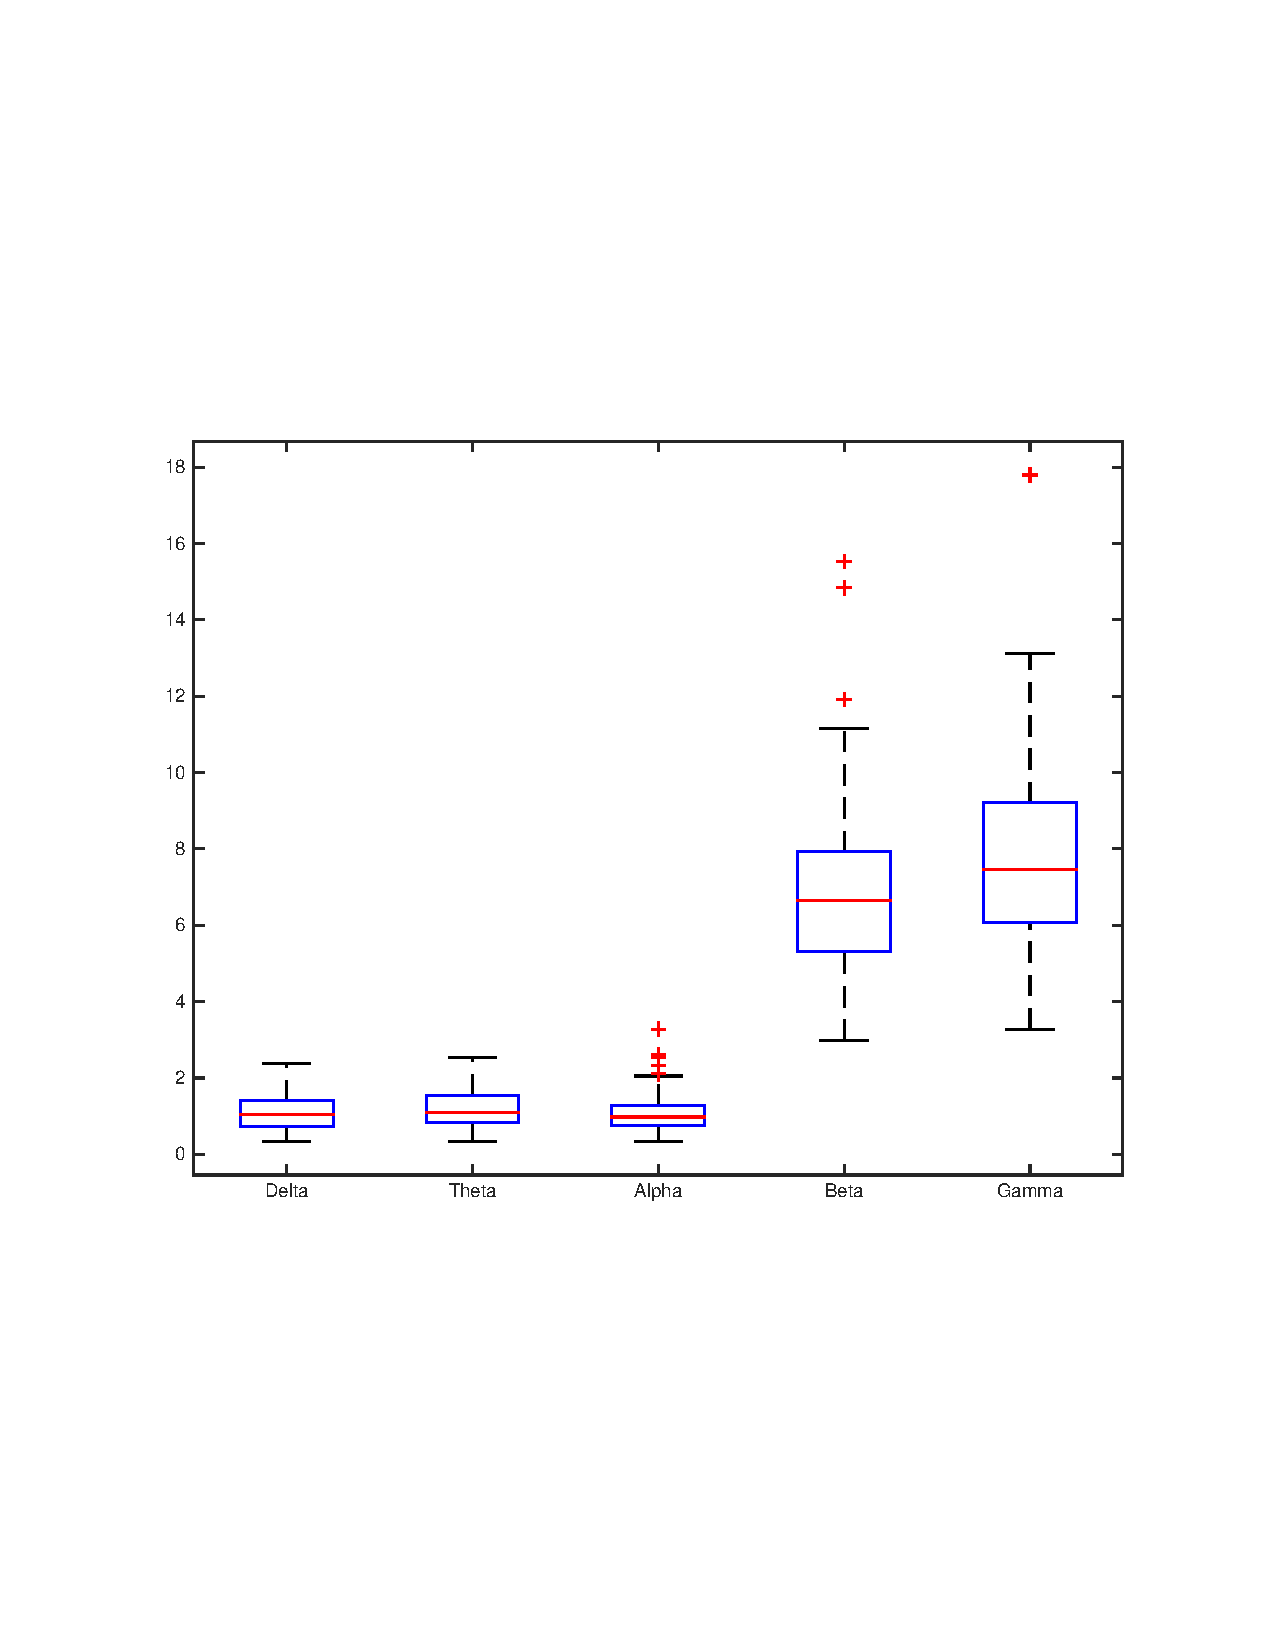
\includegraphics[scale=0.4]{14energy_band.pdf}
\label{fig:subfigure151}}
\quad
\subfigure[Compressive Sensing]{%
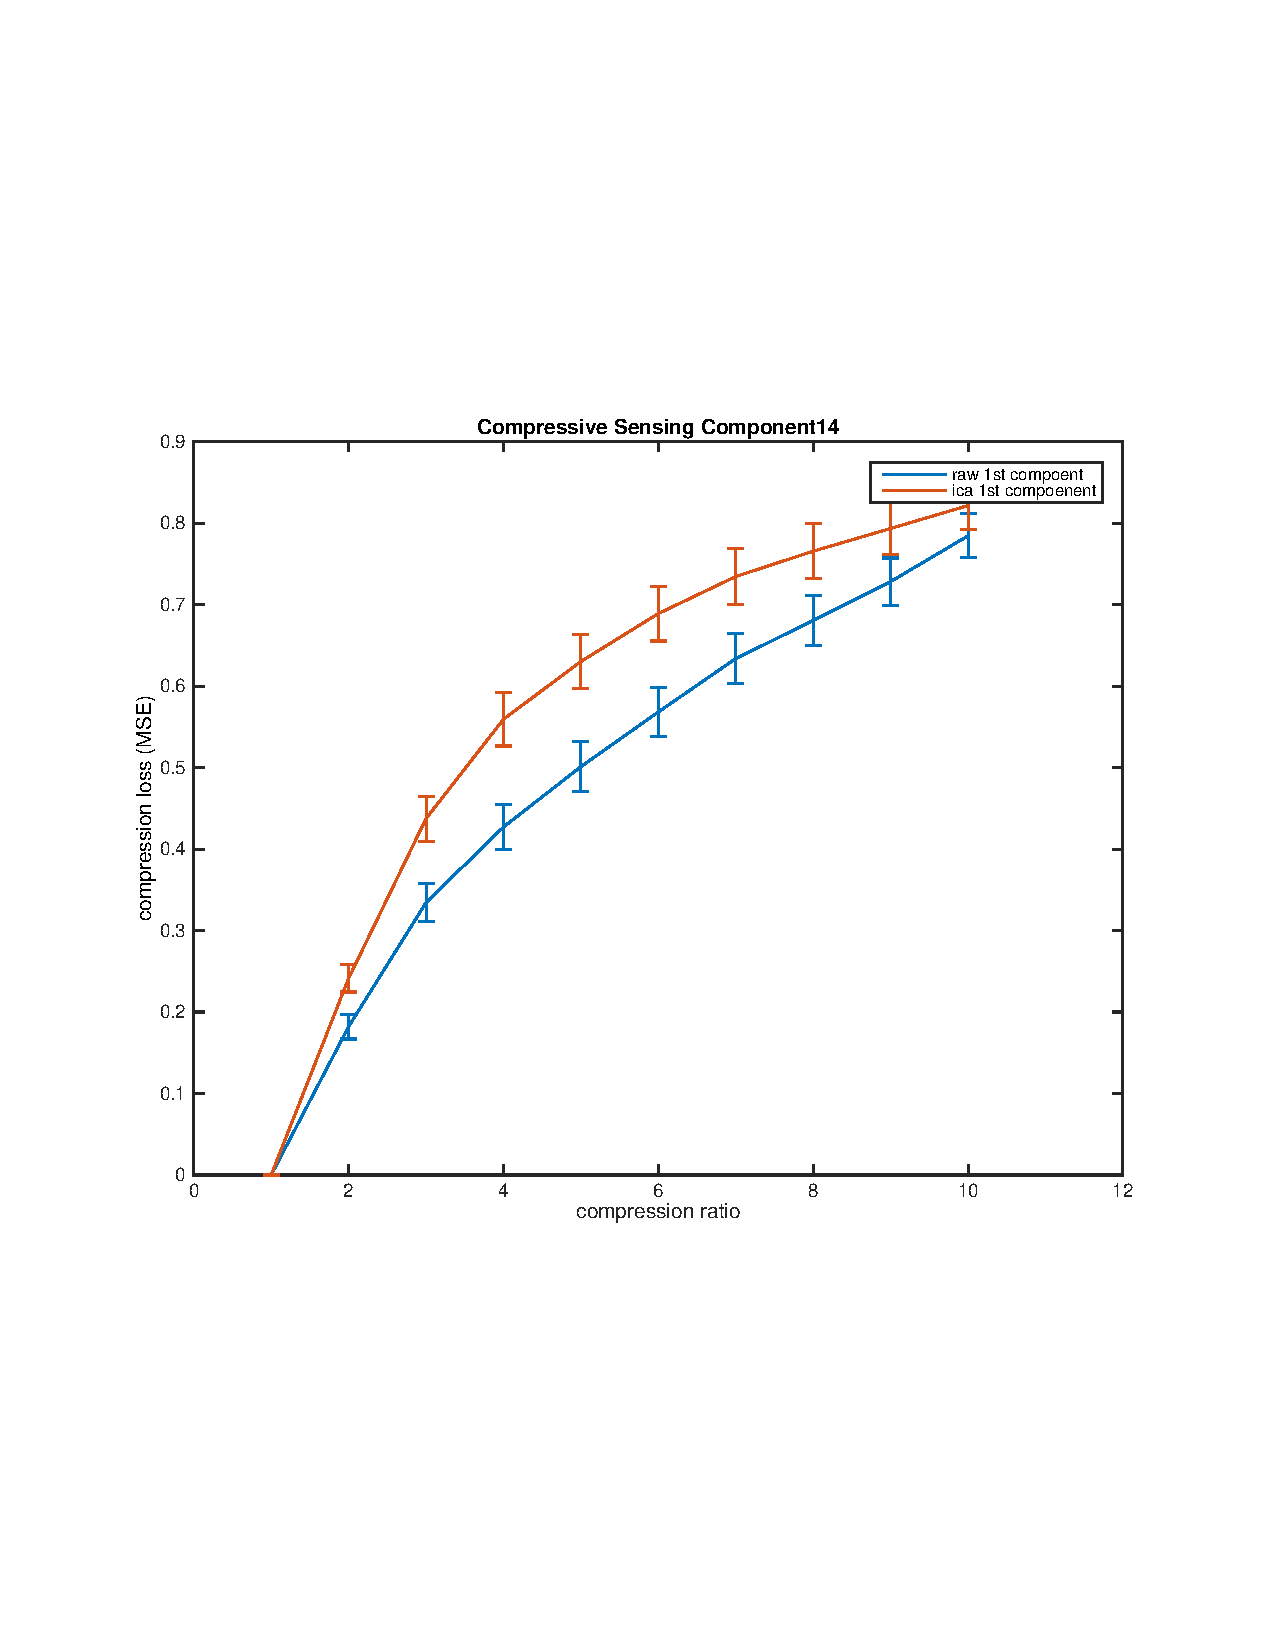
\includegraphics[scale=0.4]{comp_sen_14}
\label{fig:subfigure152}}
\subfigure[Scalp]{%
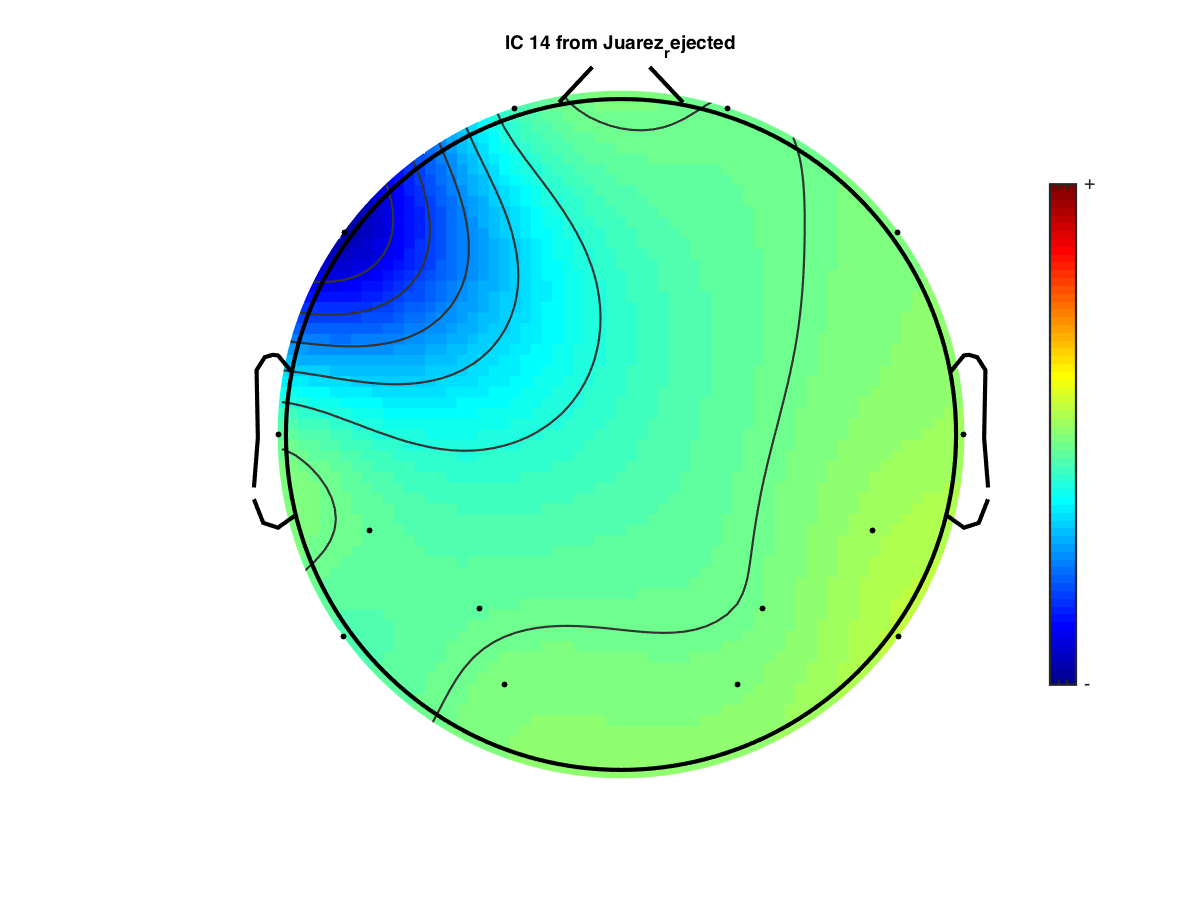
\includegraphics[scale=0.4]{ica_14}
\label{fig:subfigure153}}

%
\caption{IC 14}
\label{fig:figure15}
\end{figure}
\begin{figure}
\centering
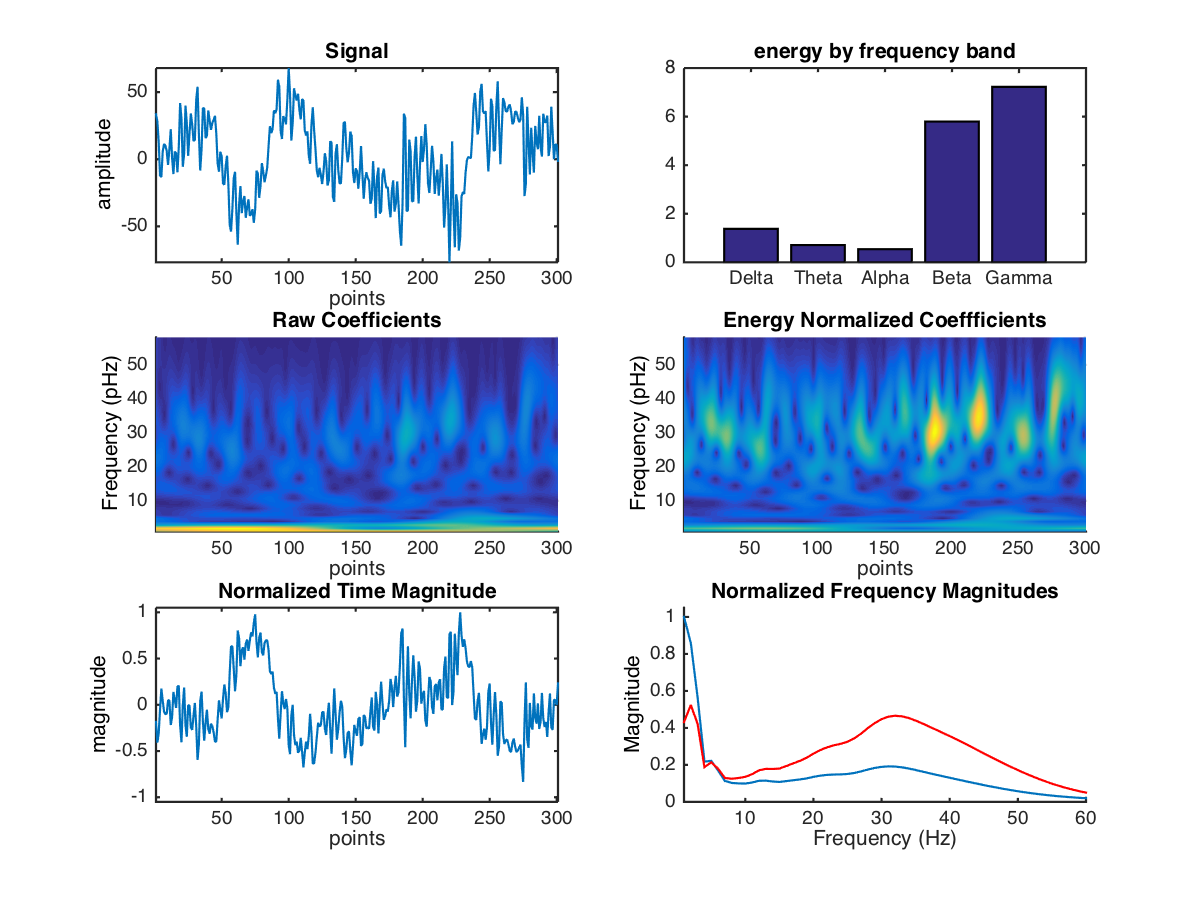
\includegraphics[width=1\textwidth]{14cwt}
\end{figure}

\end{document}